\section{Introduction}
\label{s_motive}


Nuclear expertise is rapidly expanding around the world as demand for energy increases steadily\cite{mooney_why_2014}.  As climate change becomes increasingly important with respect to national security, the perception of the risk inherent to nuclear energy is decreasing and states are embracing nuclear energy as a reliable large-scale source of carbon-neutral energy.  However, the expansion of nuclear power amplifies nuclear security concerns as the knowledge and technology required to make nuclear weapons proliferates around the globe \cite{feiveson_unmaking_2014}.  

While it has not proven possible to prevent the spread of nuclear knowledge entirely, international treaties have been used in an attempt to minimize it.  The \gls{NPT}, which has been signed by 190 states including the original five nuclear weapons states, has codified a set of rules and norms for allowing the peaceful pursuit of nuclear energy \cite{_treaty_????}.  The \gls{NPT} created the \gls{IAEA}, whose role is to verify compliance with the treaty by periodically inspecting facilities related to nuclear technology.  Other relevant treaties include \gls{CTBT}, which placed a moratorium on testing nuclear weapons, and the \gls{START} in which the \gls{US} and Russia agreed to nuclear arms reductions \cite{_treaty:_????, department_of_State_new_2010}.  A potential \gls{FMCT} would place limits on the amount of weapons-grade fissile material that each signatory state could stockpile, possibly including current stockpiles in the case of weapons states.

\begin{figure}%[htbp!]
\begin{center}
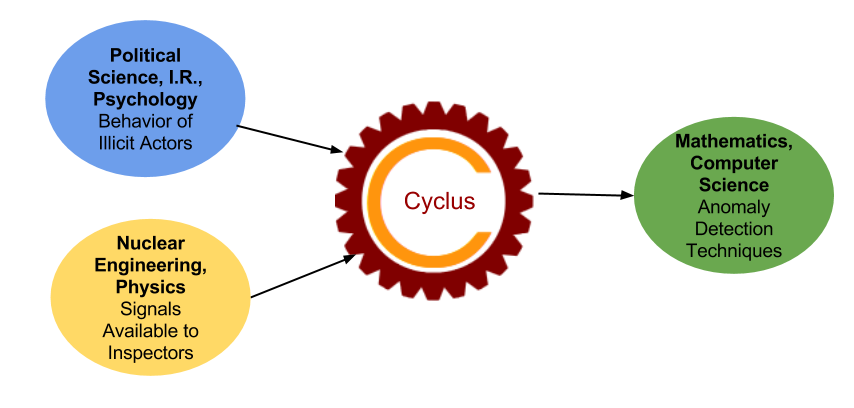
\includegraphics[natwidth=162bp,natheight=227bp, scale=0.45]{./figs/cyclus_interdiscipline.png}
\end{center}
\caption{The \Cyclus nuclear fuel cycle simulator provides a testbed to integrate innovations in treaty verification across many disciplines.}
\label{fig:cyclus_diagram}
\end{figure}

An effective treaty verification regime must synthesize knowledge from the realms of political science, international relations, nuclear physics and engineering, and even behavioral psychology.  Figure \ref{fig:cyclus_diagram} illustrates  the role of a fuel cycle simulator such as \Cyclus in bringing together these disparate fields to provide insights into proposed verification technologies. A fuel cycle simulator tracks the flow of nuclear material through the facilities in a fuel cycle\cite{huff_fundamental_2016}.  Uranium enrichment and spent fuel reprocessing are two particularly sensitive parts of the fuel cycle, but correlated signatures of illicit activity are likely to be present across the fuel cycle. A fuel cycle simulator creates synthetic data, such as what would be available to an inspector, for many different facilities simultaneously while incorporating a system-level perspective of proliferation scenarios. This synthetic data can then be used as a testbed to investigate the efficacy of new detection and analysis techniques and illucidate the strengths and weaknesses of various verification strategies.